\documentclass[10pt]{scrartcl}
% \documentclass[10pt]{article}
\usepackage[T1]{fontenc}
\usepackage{amsmath,amsfonts,amssymb}
\usepackage{mathtools}
\usepackage{color,soul}
\usepackage{fullpage}
\usepackage{enumerate}
\usepackage{graphicx}
\usepackage[colorlinks=true,urlcolor=blue]{hyperref}
\usepackage{caption}
\usepackage{subcaption}
\usepackage{deluxetable}
\usepackage{verbatim}
\usepackage{fancyvrb}
\usepackage{listings}
\usepackage{acronym}
\usepackage{amsthm} % Uuhhh yet another package


\definecolor{Light}{gray}{.90}
\sethlcolor{Light}

\lstset{%
language=C++,                   % choose the language of the code
basicstyle=\footnotesize\sffamily,%\ttfamily\footnotesize,       % the size of the fonts that are used for the code
numbers=left,                   % where to put the line-numbers
numberstyle=\footnotesize,      % the size of the fonts that are used for the line-numbers
stepnumber=1,                   % the step between two line-numbers. If it is 1 each line will be numbered
numbersep=5pt,                  % how far the line-numbers are from the code
showspaces=false,               % show spaces adding particular underscores
showstringspaces=false,         % underline spaces within strings
showtabs=false,                 % show tabs within strings adding particular underscores
% frame=single,                   % adds a frame around the code
backgroundcolor=\color{Light},
columns=fullflexible,
tabsize=2,                      % sets default tabsize to 2 spaces
captionpos=b,                   % sets the caption-position to bottom
breaklines=true,                % sets automatic line breaking
breakatwhitespace=false,        % sets if automatic breaks should only happen at whitespace
escapeinside={\%*}{*)}          % if you want to add a comment within your code
}


\title{Notes on Current Method Applied to New Grainy Image}
\author{Jeren Suzuki}
\date{Last Edited \today}

\begin{document}

\maketitle
\pagenumbering{Roman}
\tableofcontents
\clearpage
\pagenumbering{arabic}

\section{Introduction} % (fold)
Using a new test image, we see how robust our method is applied to a different (and most likely more realistic) image. The new image measures 1296 x 966 in size, compared to out old image size of 449 x 321. The result is that out image runs slower, but not linearly so. \\

\begin{figure}[!ht]
    \centering
    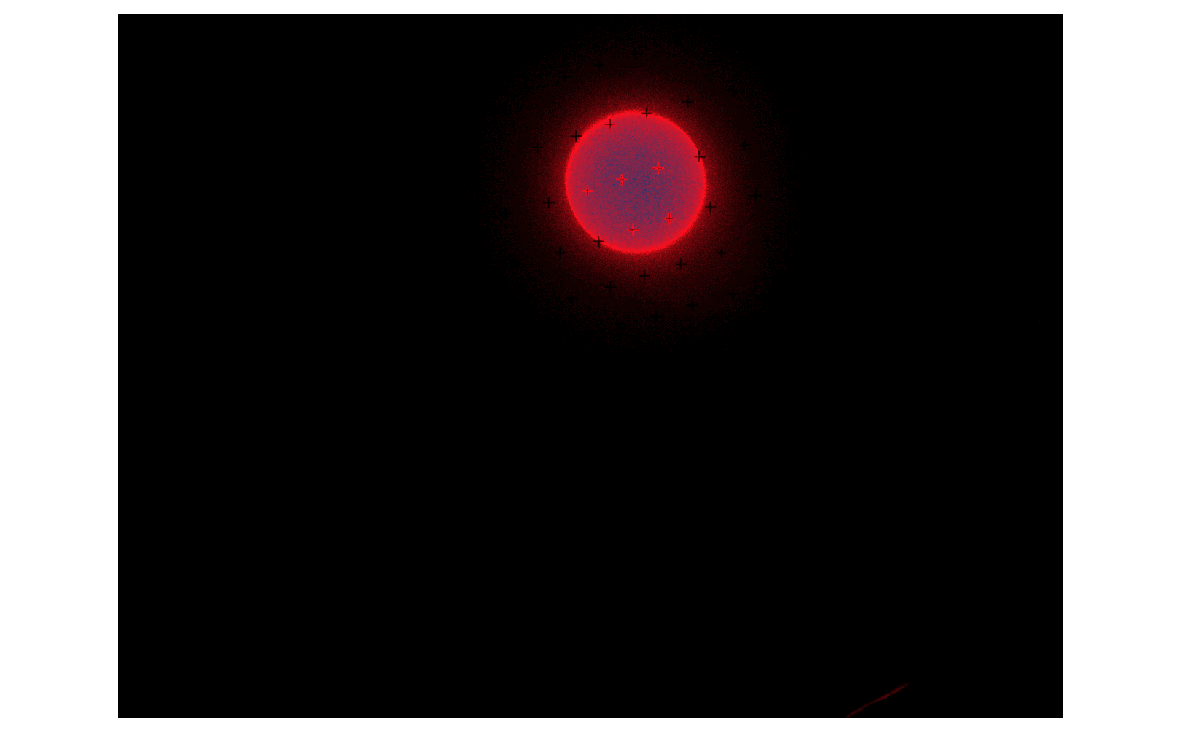
\includegraphics[width=.9\textwidth]{../plots_tables_images/grainysun.eps}    
    \caption{I have used a different color table here (Stern Special) because the black and white image was too dim. The fiducials are staggered and can be seen extending off the solar limbs.}
    \label{grainy}
\end{figure}

% section introduction (end)

\section{How Slow is Slow} % (fold)
\label{sec:how_slow_is_slow}
Table \ref{slow} lays out where our code takes the most time. Part of the process of making the code faster will be looking at which routines are called sparsely but still consume a lot of computing time, like \hl{\texttt{sort()}}, for example.

\begin{deluxetable}{rrrrr}
\tablecaption{Time (Total elapsed: 0.23658586 s)}
\tabletypesize{\scriptsize}
\tablewidth{0pt}
\tablehead{
    \colhead{Routine} %
&   \colhead{Times Called} %
&   \colhead{Time Taken} %
&   \colhead{Time Taken} %
&   \colhead{A Number} %
}
\startdata
SORT                &     64  &  0.02678 & 0.02678 & 1\\
CONVOL              &      1  &  0.02617 & 0.02617 & 1\\
SMOOTH              &      2  &  0.01668 & 0.01668 & 1\\
ROTATE              &      5  &  0.01565 & 0.01565 & 1\\
SHIFT               &      8  &  0.00713 & 0.00713 & 1\\
HISTOGRAM           &      2  &  0.00706 & 0.00706 & 1\\
LABEL\_REGION        &      2  &  0.00641 & 0.00641 & 1\\
ERODE               &      2  &  0.00385 & 0.00385 & 1\\
TOTAL               &    141  &  0.00318 & 0.00318 & 1\\
DILATE              &      2  &  0.00262 & 0.00262 & 1\\
FLOAT               &    121  &  0.00200 & 0.00200 & 1\\
WHERE               &     38  &  0.00161 & 0.00161 & 1\\
MAX                 &     10  &  0.00087 & 0.00087 & 1\\
RESOLVE\_ROUTINE     &      1  &  0.00026 & 0.00026 & 1\\
BYTARR              &     10  &  0.00018 & 0.00018 & 1\\
REPLICATE           &     14  &  0.00006 & 0.00006 & 1\\
STRTRIM             &     50  &  0.00005 & 0.00005 & 1\\
FIX                 &     21  &  0.00005 & 0.00005 & 1\\
FINDGEN             &      8  &  0.00004 & 0.00004 & 1\\
READF               &     10  &  0.00003 & 0.00003 & 1\\
PROFILER            &      1  &  0.00003 & 0.00003 & 1\\
CREATE\_STRUCT       &     11  &  0.00003 & 0.00003 & 1\\
ON\_ERROR            &     73  &  0.00003 & 0.00003 & 1\\
STRMID              &     34  &  0.00002 & 0.00002 & 1\\
FILE\_LINES          &      1  &  0.00002 & 0.00002 & 1\\
GETTOK              &      2  &  0.00001 & 0.00002 & 0\\
STRTOK              &     10  &  0.00002 & 0.00002 & 1\\
REFORM              &     39  &  0.00002 & 0.00002 & 1\\
FLTARR              &     19  &  0.00002 & 0.00002 & 1\\
SQRT                &     62  &  0.00002 & 0.00002 & 1\\
SCOPE\_VARFETCH      &     12  &  0.00002 & 0.00002 & 1\\
STRCOMPRESS         &     12  &  0.00002 & 0.00002 & 1\\
DOUBLE              &     10  &  0.00001 & 0.00001 & 1\\
OPENR               &      1  &  0.00001 & 0.00001 & 1\\
N\_PARAMS            &     36  &  0.00001 & 0.00001 & 1\\
PRINT               &      1  &  0.00001 & 0.00001 & 1\\
INDGEN              &      3  &  0.00001 & 0.00001 & 1\\
MIN                 &      8  &  0.00001 & 0.00001 & 1\\
FINITE              &     12  &  0.00001 & 0.00001 & 1\\
MESSAGE             &      1  &  0.00001 & 0.00001 & 1\\
DEFSYSV             &      2  &  0.00001 & 0.00001 & 1\\
STRING              &     12  &  0.00001 & 0.00001 & 1\\
STRLEN              &     30  &  0.00001 & 0.00001 & 1\\
FREE\_LUN            &      1  &  0.00001 & 0.00001 & 1\\
CATCH               &     10  &  0.00001 & 0.00001 & 1\\
PRODUCT             &      5  &  0.00000 & 0.00000 & 1\\
ARRAY\_EQUAL         &      5  &  0.00000 & 0.00000 & 1\\
BYTE                &      4  &  0.00000 & 0.00000 & 1\\
MAKE\_ARRAY          &      2  &  0.00000 & 0.00000 & 1\\
SYSTIME             &      2  &  0.00000 & 0.00000 & 1\\
STRPOS              &      3  &  0.00000 & 0.00000 & 1\\
ABS                 &     13  &  0.00000 & 0.00000 & 1\\
TAG\_NAMES           &      1  &  0.00000 & 0.00000 & 1\\
ISA                 &      9  &  0.00000 & 0.00000 & 1\\
SKIP\_LUN            &      1  &  0.00000 & 0.00000 & 1\\
PTR\_FREE            &      1  &  0.00000 & 0.00000 & 1\\
PTR\_NEW             &      2  &  0.00000 & 0.00000 & 1\\
PTRARR              &      1  &  0.00000 & 0.00000 & 1\\
STRUPCASE           &      1  &  0.00000 & 0.00000 & 1\\
INTARR              &      1  &  0.00000 & 0.00000 & 1
\enddata
\label{slow}
\end{deluxetable}

% section how_slow_is_slow (end)

\section{Code Flow Chart} % (fold)
\label{sec:code_flow_chart}

\begin{figure}[!ht]
    \centering
    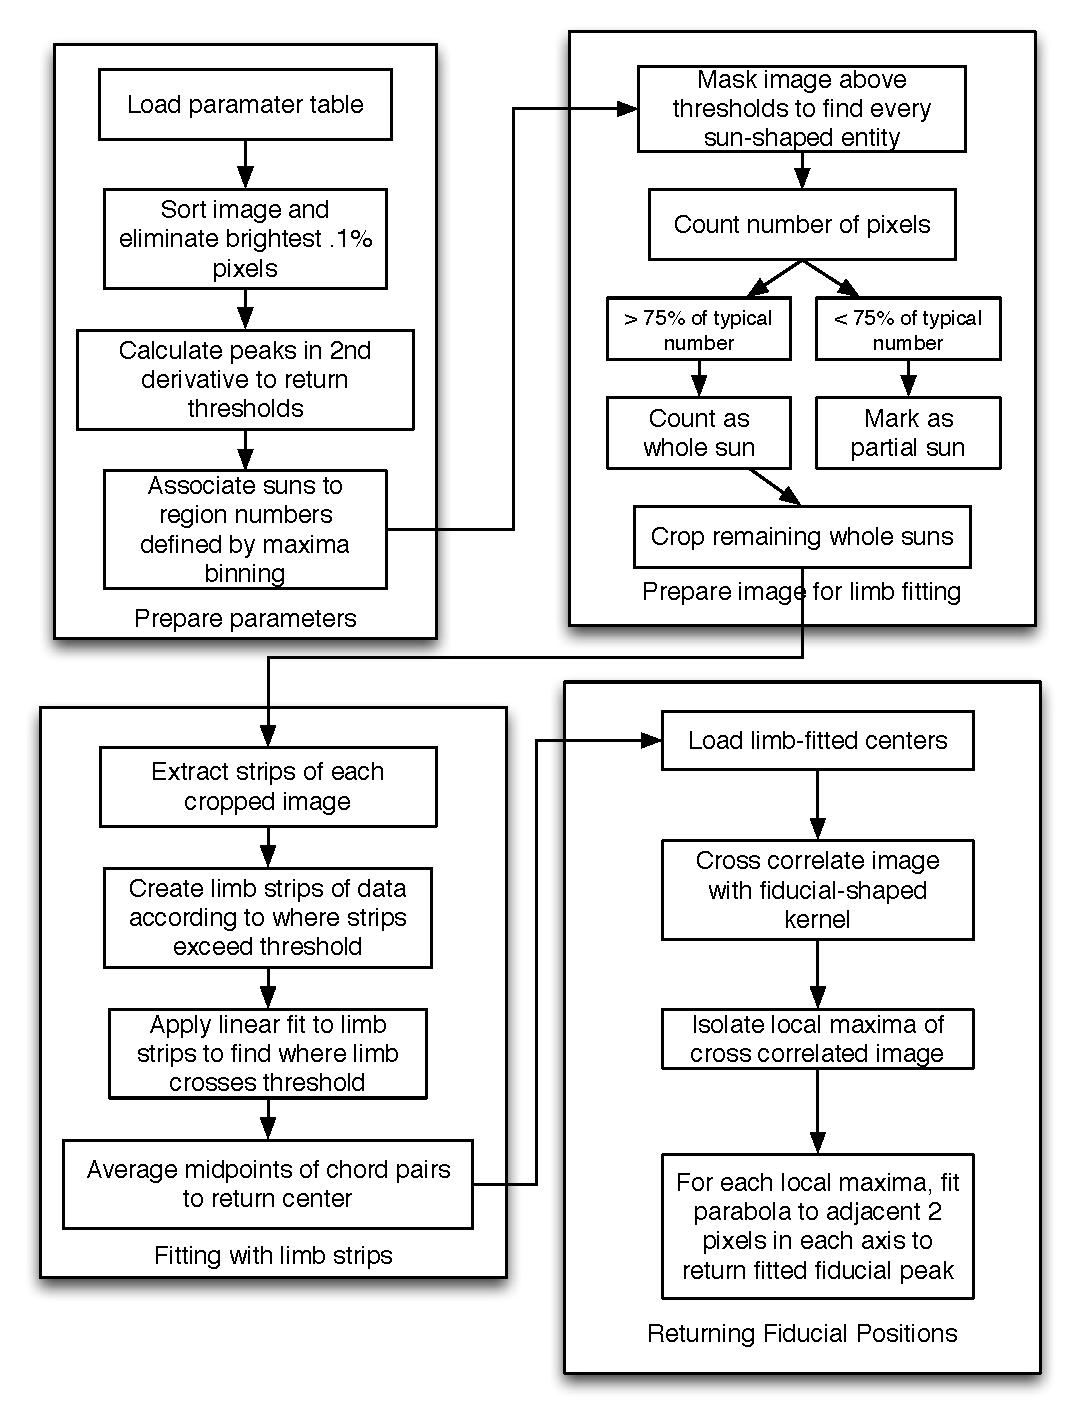
\includegraphics[width=.9\textwidth]{../plots_tables_images/alpha_flow.eps}    
    \caption{}
    \label{aflow}
\end{figure}

% section code_flow_chart (end)

% \newpage
\clearpage

\section{The Dreaded Nested For Loop} % (fold)
\label{sec:the_dreaded_nested_for_loop}
This is taken straight from Albert's C++ code:

\begin{lstlisting}
for (int m = 1; m < correlation.rows-1; m++)
    {
        for (int n = 1; n < correlation.cols-1; n++)
        {        
            thisValue = correlation.at<float>(m,n);
            if(thisValue > threshold)
            {
                //Checks if cross correlated pixel is higher than adjacent pixels                
                if((thisValue > correlation.at<float>(m, n + 1)) &
                   (thisValue > correlation.at<float>(m, n - 1)) &
                   (thisValue > correlation.at<float>(m + 1, n)) &
                   (thisValue > correlation.at<float>(m - 1, n)))
                {
                    redundant = false;
                    for (unsigned int k = 0; k <  pixelFiducials.size(); k++)
                    {
                        // Checks if previous fiducial correlation values are within 2 fiducial lengths of each other. If so, use the one with a higher correlation value
                        if (abs(pixelFiducials[k].y - m) < fiducialLength*2 &&
                            abs(pixelFiducials[k].x - n) < fiducialLength*2)
                        {
                            redundant = true;
                            thatValue = correlation.at<float>((int) pixelFiducials[k].y,(int) pixelFiducials[k].x);
                            Choose the "fiducial" with a higher correlation value
                            if ( thisValue > thatValue)
                            {
                                pixelFiducials[k] = cv::Point2f(n,m);
                            }
                            // Break out of this because there should only be one instance of this per run
                            break;
                        }
                    }
                    // Regardless of whether or not the fiducial was replaced, break out of the loop
                    if (redundant == true)
                        continue;

                    // If we're short a few entries for fiducials, extend the array
                    if ( (int) pixelFiducials.size() < numFiducials)
                    {
                        pixelFiducials.add(n, m);
                    }
                    else
                    {
                        // Dealing with too many fiducials
                        minValue = std::numeric_limits<float>::infinity();;
                        minIndex = -1;
                        for (int k = 0; k < numFiducials; k++)
                        {
                            if (correlation.at<float>((int) pixelFiducials[k].y,(int) pixelFiducials[k].x) 
                                < minValue)
                            {
                                minIndex = k;
                                minValue = correlation.at<float>((int) pixelFiducials[k].y,(int) pixelFiducials[k].x);
                            }   
                        }
                        if (thisValue > minValue)
                        {
                            pixelFiducials[minIndex] = cv::Point2f(n, m);
                        }
                    }
                }
            }
        }
    }
\end{lstlisting}


% section the_dreaded_nested_for_loop (end)

\clearpage

\section{Comparison to Albert's Code} % (fold)
\label{sec:comparison_to_albert_s_code}

\begin{figure} [!ht]
    \centering
    \hspace{-1.0in}
    \begin{subfigure}[b]{.45\linewidth}
        \centering
        \includegraphics[width=1.3\textwidth]{../plots_tables_images/myfid.eps}
        \caption{The fiducials I find}
    \end{subfigure}
    \hspace{.5in}
    \begin{subfigure}[b]{.45\linewidth}
        \centering
        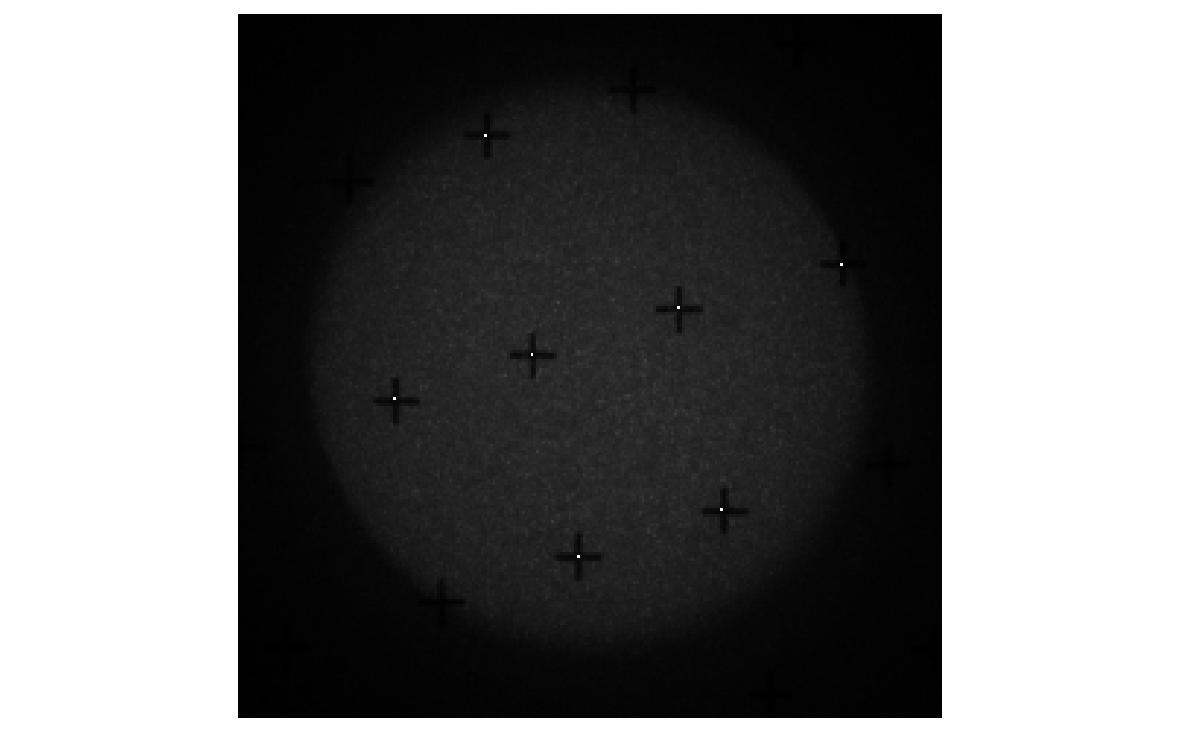
\includegraphics[width=1.3\textwidth]{../plots_tables_images/albfid.eps}
        \caption{The fiducials Albert finds}
    \end{subfigure}
    \caption{My code can't pick up two fiducials due to one or many of the following factors: different kernel, different convolution method, different threshold.}
    \label{comp}
\end{figure}

\begin{deluxetable}{rrrrr}
\tablecaption{Comparison of Fiducial Positions}
\tabletypesize{\scriptsize}
\tablewidth{0pt}
\tablehead{
    \colhead{Fiducial Number} %
&   \colhead{Albert's X} %
&   \colhead{My X} %
&   \colhead{Albert's Y} %
&   \colhead{My Y} %
}
\startdata
0 & 674.6796 & N/A & 151.0038 & N/A\\
1 & 796.3074 & N/A & 195.0324 & N/A\\
2 & 740.4443 & 741.185 & 210.6342 & 211.289\\             
3 & 690.2598 & 690.985 & 226.1973 & 226.961\\                      
4 & 643.4235 & 644.227 & 241.8869 & 242.636\\
5 & 755.8672 & 756.764 & 279.6622 & 280.443\\                                  
6 & 706.0065 & 706.809 & 295.3022 & 295.957
\enddata
\label{fidpos}
\end{deluxetable}

In Table \ref{fidpos} The fiducial positions are typically within 1 pixel of Albert's calculated positions, which is pretty good.
% section comparison_to_albert_s_code (end)

\section{Partial Sun Checking} % (fold)
\label{sec:partial_sun_checking}

We're motivated to keep some center data regardless of how cut off a sun may be. To do this, we must quantify the poorness of the fit as more sun is cut off. Figures \ref{croptestside} and \ref{croptestcorner} aim to quantify the worsening of the evaluated centers. We start by lining up the edge of the image to the solar limb then cropping in 10 columns. \\

The whole solar image consists of 26,597 pixels above the threshold.
\begin{figure}[!ht]
    \centering
    \includegraphics[width=.9\textwidth]{../plots_tables_images/cutofftestside.eps}    
    \caption{The green pixel is the image's true center and the red pixel is the center of the cropped image. The images are cropped 10 columns at a time.}
    \label{crop9side}
\end{figure}
\begin{figure}[!ht]
    \centering
    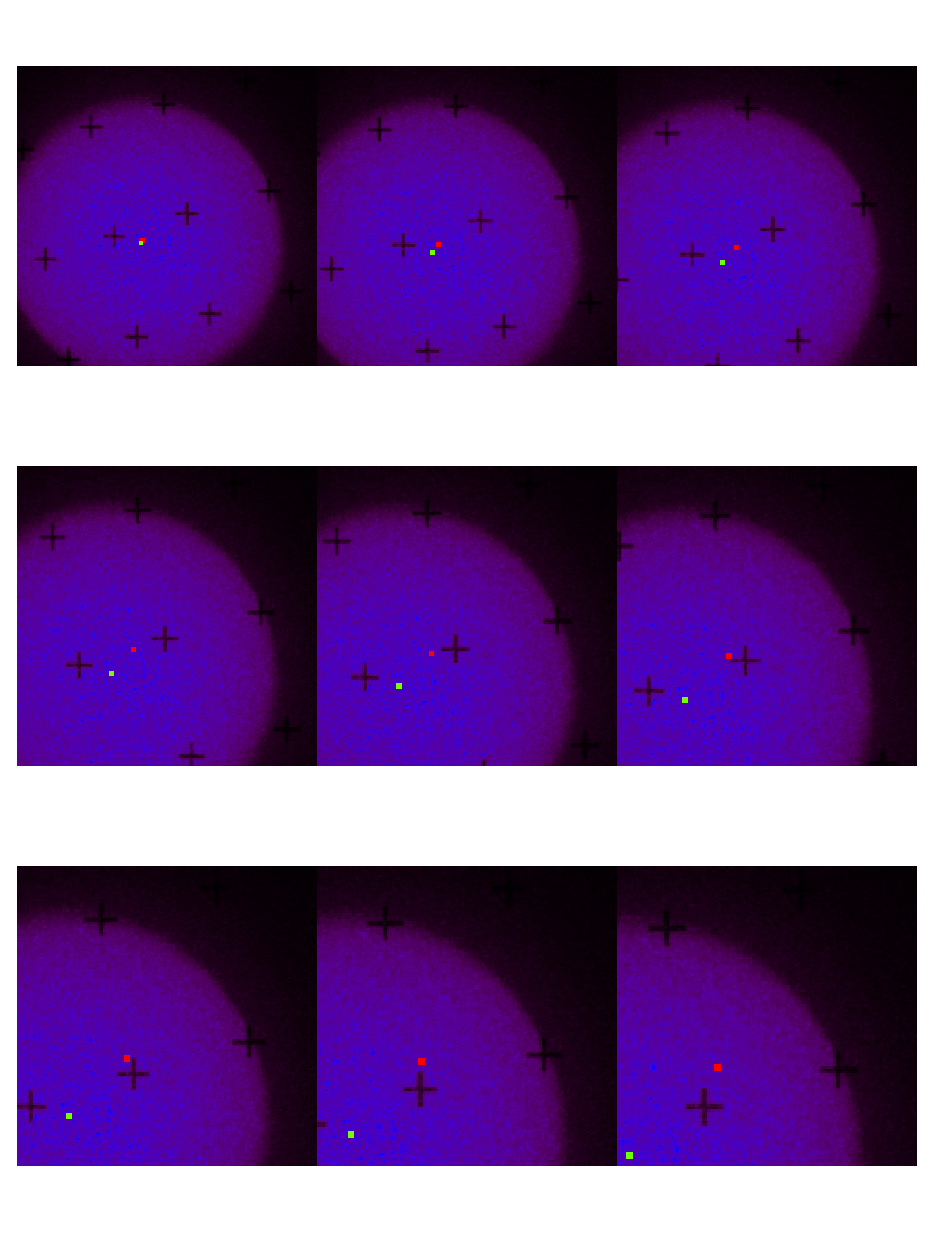
\includegraphics[width=.9\textwidth]{../plots_tables_images/cutofftestcorner.eps}    
    \caption{The green pixel is the image's true center and the red pixel is the center of the cropped image. The images are cropped 10 columns at a time.}
    \label{crop9corner}
\end{figure}

\begin{deluxetable}{crr}
\tablecaption{Side Crop Test for Figure \ref{crop9side}}
\tabletypesize{\scriptsize}
\tablewidth{0pt}
\tablehead{
    \colhead{Amount Cropped from Limb (pixels)} %
&   \colhead{$x_\textrm{True} - x_{\textrm{Cropped}}$} %
&   \colhead{$y_\textrm{True} - y_{\textrm{Cropped}}$} %
}
\startdata
10 & -1.17771 & -0.0108643 \\
20 & -4.07970 & -0.0376663 \\
30 & -7.63260 & -0.0522766 \\
40 & -11.7287 & -0.0585175 \\
50 & -16.2043 & -0.0185776 \\
60 & -20.9117 & -0.0872879 \\
70 & -25.7588 & -0.277687 \\
80 & -30.8586 & -0.321724 \\
90 & -36.1318 & -0.318489
\enddata
\label{cpos}
\end{deluxetable}

\begin{deluxetable}{crr}
\tablecaption{Corner Crop Test for Figure \ref{crop9corner}}
\tabletypesize{\scriptsize}
\tablewidth{0pt}
\tablehead{
    \colhead{Amount Cropped from Limb (pixels)} %
&   \colhead{$x_\textrm{True} - x_{\textrm{Cropped}}$} %
&   \colhead{$y_\textrm{True} - y_{\textrm{Cropped}}$} %
}
\startdata
10 & -1.17902 & -1.22132 \\
20 & -4.23825 & -4.28215 \\
30 & -8.41805 & -8.49775 \\
40 & -13.2540 & -13.3160 \\
50 & -18.2548 & -18.0202 \\
60 & -23.0267 & -22.9181 \\
70 & -27.5755 & -27.8987 \\
80 & -32.1102 & -32.4790 \\
90 & -36.6139 & -37.0980
\enddata
\label{ccpos}
\end{deluxetable}

\begin{figure}[!ht]
    \centering
    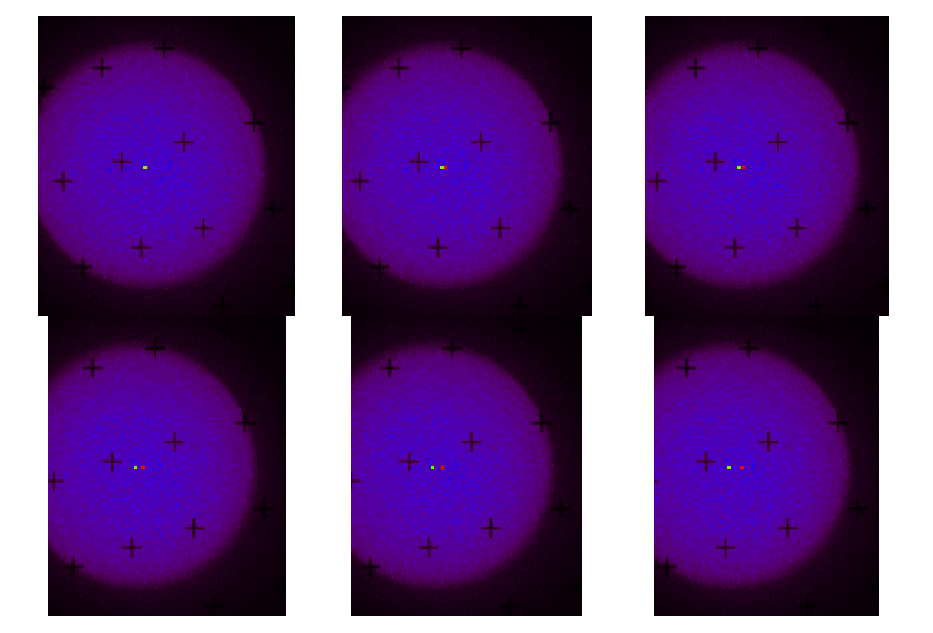
\includegraphics[width=.9\textwidth]{../plots_tables_images/side5col.eps}
    \caption{The sun is being cropped off 5 columns at a time, opposed to the earlier Figures' 10.}
    \label{croptestside}
\end{figure}
\begin{figure}[!ht]
    \centering
    \includegraphics[width=.9\textwidth]{../plots_tables_images/diag5col.eps}
    \caption{}
    \label{croptestcorner}
\end{figure}

\begin{deluxetable}{crrrr}
\tablecaption{Side Crop Test for Figure \ref{croptestside}}
\tabletypesize{\scriptsize}
\tablewidth{0pt}
\tablehead{
    \colhead{Amount Cropped from Limb (pixels)} %
&   \colhead{$x_\textrm{True} - x_{\textrm{Cropped}}$} %
&   \colhead{$y_\textrm{True} - y_{\textrm{Cropped}}$} %
&   \colhead{$N_{\textrm{pixels}}$ above threshold} %
&   \colhead{Percentage of Total Pixels} %
}
\startdata
5  & -1.17771 & -0.0108643 & 26250 & 98.6953\\
10 & -2.52845 & -0.0205002 & 25838 & 97.1463\\
15 & -4.07970 & -0.0376663 & 25353 & 95.3228\\
20 & -5.82758 & -0.0490799 & 24795 & 93.2248\\
25 & -7.63260 & -0.0522766 & 24208 & 91.0178\\
30 & -9.60011 & -0.0380630 & 23557 & 88.5701
\enddata
\label{ccpos}
\end{deluxetable}



\begin{deluxetable}{crrrr}
\tablecaption{Corner Crop Test for Figure \ref{croptestcorner}}
\tabletypesize{\scriptsize}
\tablewidth{0pt}
\tablehead{
    \colhead{Amount Cropped from Limb (pixels)} %
&   \colhead{$x_\textrm{True} - x_{\textrm{Cropped}}$} %
&   \colhead{$y_\textrm{True} - y_{\textrm{Cropped}}$} %
&   \colhead{$N_{\textrm{pixels}}$ above threshold} %
&   \colhead{Percentage of Total Pixels} %
}
\startdata
5  & -1.17902 & -1.22132 & 25896 & 97.3644 \\
10 & -2.58559 & -2.60790 & 25079 & 94.2926 \\
15 & -4.23825 & -4.28215 & 24113 & 90.6606 \\
20 & -6.22114 & -6.27864 & 22994 & 86.4534 \\
25 & -8.41805 & -8.49775 & 21805 & 81.9829 \\
30 & -10.8070 & -10.8650 & 20544 & 77.2418
\enddata
\label{ccpos}
\end{deluxetable}

% section partial_sun_checking (end)

\section{Glaring Problems} % (fold)
\label{sec:glaring_problems}
I was having trouble with proper thresholding but it was alleviated with increasing the smoothing parameter. \emph{Go parameter block!}\\

Our attempts to identify partial suns has evolved from:

\begin{enumerate}
    \item Determining if center of sun is within certain distance of border
    \item Count pixels on very border of image, if 6 consecutive pixels found, mark nearest sun as partial
    \item Count number of solar pixels above threshold, if below a certain amount, marked as partial sun
\end{enumerate}

The problem with the second method is that the shape of our mask is designed such that the bottom two corners will always be dark so scanning in a border-pattern will return ill results. We've opted to return to the first method, masking the sun, regardless of shape, and measuring the distance between the mask center and the edge of the image. 

\begin{figure}[!ht]
    \centering
    \hspace{-1.0in}
    \begin{subfigure}[b]{.45\linewidth}
        \centering
        
\includegraphics[width=1.3\textwidth]{../plots_tables_images/cutcorner.eps}
        \caption{What our mask should look like - side of black triangle is 1/4 of image width}
        \label{noborder}
    \end{subfigure}
    \hspace{.5in}
    \begin{subfigure}[b]{.45\linewidth}
        \centering
        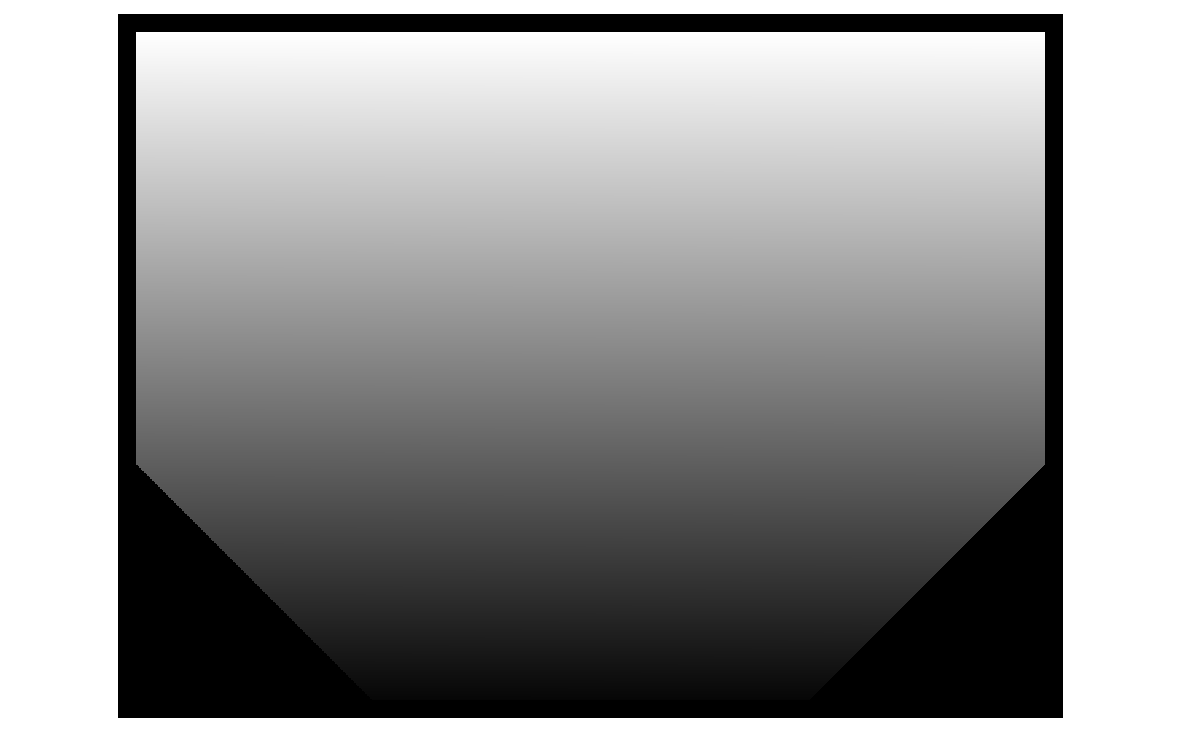
\includegraphics[width=1.3\textwidth]{../plots_tables_images/cutcornerwborder.eps}
        \caption{A proposed mask that looks within a certain distance form the border.}
        \label{aborder}
    \end{subfigure}
    \caption{The problem with the mask in \ref{aborder} is that we use an erode function (\emph{which takes an ungodly amount of time}) to shrink the mask used in \ref{noborder}.}
    \label{cuttingcorners}
\end{figure}

A possible approach is to use the mask in Figure \ref{noborder} and check the distance to the closest non-0 pixel; the problem with this method are the numerous \hl{\texttt{sqrt()}} calls to each pixel on the border of our image. 

\begin{deluxetable}{lrr}
\tablecaption{Comparison of Center Positions}
\tabletypesize{\scriptsize}
\tablewidth{0pt}
\tablehead{
    \colhead{Method} %
&   \colhead{X Position} %
&   \colhead{Y Position} %
}
\startdata
Mine & 710.811 & 230.695\\
Albert's & 709.7835 & 230.1023
\enddata
\label{cpos}
\end{deluxetable}


% section glaring_problems (end)

\end{document}










